\documentclass[12pt]{article}
\usepackage{tikz}

\begin{document}

\begin{center}
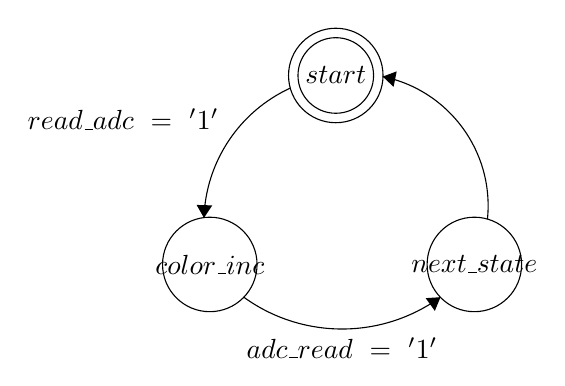
\begin{tikzpicture}[scale=0.2]
\tikzstyle{every node}+=[inner sep=0pt]
\draw [black] (34.4,-17) circle (3);
\draw (34.4,-17) node {$start$};
\draw [black] (34.4,-17) circle (2.4);
\draw [black] (26.4,-29) circle (3);
\draw (26.4,-29) node {$color\_inc$};
\draw [black] (43.2,-29) circle (3);
\draw (43.2,-29) node {$next\_state$};
\draw [black] (26.028,-26.036) arc (-181.97204:-245.4081:9.418);
\fill [black] (26.03,-26.04) -- (26.56,-25.25) -- (25.56,-25.22);
\draw (26.99,-19.8) node [left] {$read\_adc\mbox{ }=\mbox{ }'1'$};
\draw [black] (41.048,-31.076) arc (-54.0987:-125.9013:10.655);
\fill [black] (41.05,-31.08) -- (40.11,-31.14) -- (40.69,-31.95);
\draw (34.8,-33.6) node [below] {$adc\_read\mbox{ }=\mbox{ }'1'$};
\draw [black] (37.383,-17.07) arc (78.39313:-5.88546:8.376);
\fill [black] (37.38,-17.07) -- (38.07,-17.72) -- (38.27,-16.74);
\end{tikzpicture}
\end{center}

\end{document}

